\documentclass[11pt,reqno]{book}

%%%%%%%%%%%%%%%%%%%%%%%%%%%%%%%%%%%%%%%%%
% The Legrand Orange Book
% Structural Definitions File
% Version 2.1 (26/09/2018)
%
% Original author:
% Mathias Legrand (legrand.mathias@gmail.com) with modifications by:
% Vel (vel@latextemplates.com)
% 
% This file was downloaded from:
% http://www.LaTeXTemplates.com
%
% License:
% CC BY-NC-SA 3.0 (http://creativecommons.org/licenses/by-nc-sa/3.0/)
%
%%%%%%%%%%%%%%%%%%%%%%%%%%%%%%%%%%%%%%%%%

%---------------------------------------------------------------------
%	VARIOUS REQUIRED PACKAGES AND CONFIGURATIONS
%---------------------------------------------------------------------
\usepackage{comment}
\usepackage{graphicx} % Required for including pictures
\graphicspath{{Pictures/}} 
\usepackage{lipsum} % Inserts dummy text

% Required for drawing custom shapes
\usepackage{tikz} 
\usetikzlibrary{shadows}
\usetikzlibrary{fadings}
\usepackage{tcolorbox}
\tcbuselibrary{skins}
\definecolor{mygreen}{RGB}{0, 128, 0}
\usepackage{subfigure}
\usepackage{float}


\usepackage[portuguese]{babel} % English language/hyphenation
\usepackage{enumitem} % Customize lists
\setlist{nolistsep} 
\usepackage{booktabs} % Required for nicer horizontal rules in tables
\usepackage{xcolor} % Required for specifying colors by name
\definecolor{ocre}{RGB}{29,152,66} 
\definecolor{chapterhead}{RGB}{14,69,31}
\usepackage{sectsty} %CHange Color for Headings
\usepackage{indentfirst}
\usepackage{graphicx,wrapfig}
\usepackage[pt-BR]{datetime2}


%---------------------------------------------------------------------
%	MARGINS
%---------------------------------------------------------------------

\usepackage{geometry} % Required for adjusting page dimensions and margins

\geometry{
	paper=a4paper, % Paper size, change to letterpaper for US letter size
	top=3cm, % Top margin
	bottom=2cm, % Bottom margin
	left=3cm, % Left margin
	right=2cm, % Right margin
	headheight=14pt, % Header height
	footskip=1.4cm, % Space from the bottom margin to the baseline of the footer
	headsep=10pt, % Space from the top margin to the baseline of the header
}

%---------------------------------------------------------------------
%	FONTS
%---------------------------------------------------------------------

\usepackage{avant} % Use the Avantgarde font for headings
%\usepackage{times} % Use the Times font for headings
\usepackage{mathptmx} % Use the Adobe Times Roman as the default text font together with math symbols from the Sym­bol, Chancery and Com­puter Modern fonts

\usepackage{microtype} % Slightly tweak font spacing for aesthetics
\usepackage[utf8]{inputenc} % Required for including letters with accents
\usepackage[T1]{fontenc} % Use 8-bit encoding that has 256 glyphs
\usepackage{setspace}
\usepackage{csquotes}

%---------------------------------------------------------------------
%	BIBLIOGRAPHY AND INDEX
%---------------------------------------------------------------------

\usepackage[style=numeric,citestyle=numeric,sorting=nyt,sortcites=true,autopunct=true,hyperref=true,abbreviate=false,backref=true,backend=biber]{biblatex}
\addbibresource{bibliography.bib} % BibTeX bibliography file
\defbibheading{bibempty}{}

\usepackage{calc} % For simpler calculation - used for spacing the index letter headings correctly
\usepackage{makeidx} % Required to make an index
\makeindex % Tells LaTeX to create the files required for indexing

%---------------------------------------------------------------------
%	MAIN TABLE OF CONTENTS
%---------------------------------------------------------------------

\usepackage{titletoc} % Required for manipulating the table of contents

\contentsmargin{0cm} % Removes the default margin

% Part text styling (this is mostly taken care of in the PART HEADINGS section of this file)
\titlecontents{part}
	[0cm] % Left indentation
	{\addvspace{20pt}\bfseries} % Spacing and font options for parts
	{}
	{}
	{}

% Chapter text styling
\titlecontents{chapter}
	[1.25cm] % Left indentation
	{\addvspace{12pt}\large\sffamily\bfseries} % Spacing and font options for chapters
	{\color{ocre!60}\contentslabel[\Large\thecontentslabel]{1.25cm}\color{ocre}} % Formatting of numbered sections of this type
	{\color{ocre}} % Formatting of numberless sections of this type
	{\color{ocre!60}\normalsize\;\titlerule*[.5pc]{.}\;\thecontentspage} % Formatting of the filler to the right of the heading and the page number

% Section text styling
\titlecontents{section}
	[1.25cm] % Left indentation
	{\addvspace{3pt}\sffamily\bfseries} % Spacing and font options for sections
	{\contentslabel[\thecontentslabel]{1.25cm}} % Formatting of numbered sections of this type
	{} % Formatting of numberless sections of this type
	{\hfill\color{black}\thecontentspage} % Formatting of the filler to the right of the heading and the page number

% Subsection text styling
\titlecontents{subsection}
	[1.25cm] % Left indentation
	{\addvspace{1pt}\sffamily\small} % Spacing and font options for subsections
	{\contentslabel[\thecontentslabel]{1.25cm}} % Formatting of numbered sections of this type
	{} % Formatting of numberless sections of this type
	{\ \titlerule*[.5pc]{.}\;\thecontentspage} % Formatting of the filler to the right of the heading and the page number

% Figure text styling
\titlecontents{figure}
	[1.25cm] % Left indentation
	{\addvspace{1pt}\sffamily\small} % Spacing and font options for figures
	{\thecontentslabel\hspace*{1em}} % Formatting of numbered sections of this type
	{} % Formatting of numberless sections of this type
	{\ \titlerule*[.5pc]{.}\;\thecontentspage} % Formatting of the filler to the right of the heading and the page number

% Table text styling
\titlecontents{table}
	[1.25cm] % Left indentation
	{\addvspace{1pt}\sffamily\small} % Spacing and font options for tables
	{\thecontentslabel\hspace*{1em}} % Formatting of numbered sections of this type
	{} % Formatting of numberless sections of this type
	{\ \titlerule*[.5pc]{.}\;\thecontentspage} % Formatting of the filler to the right of the heading and the page number

%---------------------------------------------------------------------
%	MINI TABLE OF CONTENTS IN PART HEADS
%---------------------------------------------------------------------

% Chapter text styling
\titlecontents{lchapter}
	[0em] % Left indentation
	{\addvspace{15pt}\large\sffamily\bfseries\color{white}} % Spacing and font options for chapters
	{\color{ocre}\contentslabel[\Large\thecontentslabel]{1.25cm}\color{ocre}} % Chapter number
	{}  
	{\color{ocre}\normalsize\sffamily\bfseries\;\titlerule*[.5pc]{.}\;\thecontentspage} % Page number

% Section text styling
\titlecontents{lsection}
	[0em] % Left indentation
	{\sffamily\small} % Spacing and font options for sections
	{\contentslabel[\thecontentslabel]{1.25cm}} % Section number
	{}
	{}

% Subsection text styling (note these aren't shown by default, display them by searchings this file for tocdepth and reading the commented text)
\titlecontents{lsubsection}
	[.5em] % Left indentation
	{\sffamily\footnotesize} % Spacing and font options for subsections
	{\contentslabel[\thecontentslabel]{1.25cm}}
	{}
	{}

%---------------------------------------------------------------------
%	HEADERS AND FOOTERS
%---------------------------------------------------------------------

\usepackage{fancyhdr} % Required for header and footer configuration

\pagestyle{fancy} % Enable the custom headers and footers

\pagestyle{fancy}
\renewcommand{\chaptermark}[1]{\markboth{\sffamily\normalsize\bfseries\chaptername\ \thechapter.\ #1}{}} % Chapter text font settings
 
\renewcommand{\sectionmark}[1]{\markright{\sffamily\normalsize\thesection\hspace{5pt}#1}{}} % Section text font settings
\fancyhf{} \fancyhead[LE,RO]{\sffamily\normalsize\thepage} % Font setting for the page number in the header
\fancyhead[LO]{\rightmark} % Print the nearest section name on the left side of odd pages
\fancyhead[RE]{\leftmark} % Print the current chapter name on the right side of even pages
\renewcommand{\headrulewidth}{0.5pt} % Width of the rule under the header
\addtolength{\headheight}{2.5pt} % Increase the spacing around the header slightly
\renewcommand{\footrulewidth}{0pt} % Removes the rule in the footer
\fancypagestyle{plain}{\fancyhead{}\renewcommand{\headrulewidth}{0pt}} % Style for when a plain pagestyle is specified

% Removes the header from odd empty pages at the end of chapters
\makeatletter
\renewcommand{\cleardoublepage}{
\clearpage\ifodd\c@page\else
\hbox{}
\vspace*{\fill}
\thispagestyle{empty}
\newpage
\fi}

%---------------------------------------------------------------------
%	THEOREM STYLES
%---------------------------------------------------------------------

\usepackage{amsmath,amsfonts,amssymb,amsthm} % For math equations, theorems, symbols, etc

\newcommand{\intoo}[2]{\mathopen{]}#1\,;#2\mathclose{[}}
\newcommand{\ud}{\mathop{\mathrm{{}d}}\mathopen{}}
\newcommand{\intff}[2]{\mathopen{[}#1\,;#2\mathclose{]}}
\renewcommand{\qedsymbol}{$\blacksquare$}
\newtheorem{notation}{Notação}[chapter]

% Boxed/framed environments
\newtheoremstyle{ocrenumbox}% Theorem style name
{0pt}% Space above
{0pt}% Space below
{\normalfont}% Body font
{}% Indent amount
{\small\bf\sffamily\color{ocre}}% Theorem head font
{\;}% Punctuation after theorem head
{0.25em}% Space after theorem head
{\small\sffamily\color{ocre}\thmname{#1}\nobreakspace\thmnumber{\@ifnotempty{#1}{}\@upn{#2}}% Theorem text (e.g. Theorem 2.1)
\thmnote{\nobreakspace\the\thm@notefont\sffamily\bfseries\color{black}---\nobreakspace#3.}} % Optional theorem note

\newtheoremstyle{blacknumex}% Theorem style name
{5pt}% Space above
{5pt}% Space below
{\normalfont}% Body font
{} % Indent amount
{\small\bf\sffamily}% Theorem head font
{\;}% Punctuation after theorem head
{0.25em}% Space after theorem head
{\small\sffamily{\tiny\ensuremath{\blacksquare}}\nobreakspace\thmname{#1}\nobreakspace\thmnumber{\@ifnotempty{#1}{}\@upn{#2}}% Theorem text (e.g. Theorem 2.1)
\thmnote{\nobreakspace\the\thm@notefont\sffamily\bfseries---\nobreakspace#3.}}% Optional theorem note

\newtheoremstyle{blacknumbox} % Theorem style name
{0pt}% Space above
{0pt}% Space below
{\normalfont}% Body font
{}% Indent amount
{\small\bf\sffamily}% Theorem head font
{\;}% Punctuation after theorem head
{0.25em}% Space after theorem head
{\small\sffamily\thmname{#1}\nobreakspace\thmnumber{\@ifnotempty{#1}{}\@upn{#2}}% Theorem text (e.g. Theorem 2.1)
\thmnote{\nobreakspace\the\thm@notefont\sffamily\bfseries---\nobreakspace#3.}}% Optional theorem note

% Non-boxed/non-framed environments
\newtheoremstyle{ocrenum}% Theorem style name
{5pt}% Space above
{5pt}% Space below
{\normalfont}% Body font
{}% Indent amount
{\small\bf\sffamily\color{ocre}}% Theorem head font
{\;}% Punctuation after theorem head
{0.25em}% Space after theorem head
{\small\sffamily\color{ocre}\thmname{#1}\nobreakspace\thmnumber{\@ifnotempty{#1}{}\@upn{#2}}% Theorem text (e.g. Theorem 2.1)
\thmnote{\nobreakspace\the\thm@notefont\sffamily\bfseries\color{black}---\nobreakspace#3.}} % Optional theorem note
\makeatother

% Defines the theorem text style for each type of theorem to one of the three styles above
\newcounter{dummy} 
\numberwithin{dummy}{section}
\theoremstyle{ocrenumbox}
\newtheorem{theoremeT}[dummy]{Teorema}
\newtheorem{problem}{Problema}[chapter]
\newtheorem{exerciseT}{Exercício}[chapter]
\theoremstyle{blacknumex}
\newtheorem{exampleT}{Exemplo}[chapter]
\theoremstyle{blacknumbox}
\newtheorem{vocabulary}{Vocabulário}[chapter]
\newtheorem{definitionT}{Definição}[section]
\newtheorem{corollaryT}[dummy]{Corolário}
\theoremstyle{ocrenum}
\newtheorem{proposition}[dummy]{Proposição}

%---------------------------------------------------------------------
%	DEFINITION OF COLORED BOXES
%---------------------------------------------------------------------

\RequirePackage[framemethod=default]{mdframed} % Required for creating the theorem, definition, exercise and corollary boxes

% Theorem box
\newmdenv[skipabove=7pt,
skipbelow=7pt,
backgroundcolor=black!5,
linecolor=ocre,
innerleftmargin=5pt,
innerrightmargin=5pt,
innertopmargin=5pt,
leftmargin=0cm,
rightmargin=0cm,
innerbottommargin=5pt]{tBox}

% Exercise box	  
\newmdenv[skipabove=7pt,
skipbelow=7pt,
rightline=false,
leftline=true,
topline=false,
bottomline=false,
backgroundcolor=ocre!10,
linecolor=ocre,
innerleftmargin=5pt,
innerrightmargin=5pt,
innertopmargin=5pt,
innerbottommargin=5pt,
leftmargin=0cm,
rightmargin=0cm,
linewidth=4pt]{eBox}	

% Definition box
\newmdenv[skipabove=7pt,
skipbelow=7pt,
rightline=false,
leftline=true,
topline=false,
bottomline=false,
linecolor=ocre,
innerleftmargin=5pt,
innerrightmargin=5pt,
innertopmargin=0pt,
leftmargin=0cm,
rightmargin=0cm,
linewidth=4pt,
innerbottommargin=0pt]{dBox}	

% Corollary box
\newmdenv[skipabove=7pt,
skipbelow=7pt,
rightline=false,
leftline=true,
topline=false,
bottomline=false,
linecolor=gray,
backgroundcolor=black!5,
innerleftmargin=5pt,
innerrightmargin=5pt,
innertopmargin=5pt,
leftmargin=0cm,
rightmargin=0cm,
linewidth=4pt,
innerbottommargin=5pt]{cBox}

% Creates an environment for each type of theorem and assigns it a theorem text style from the "Theorem Styles" section above and a colored box from above
\newenvironment{theorem}{\begin{tBox}\begin{theoremeT}}{\end{theoremeT}\end{tBox}}
\newenvironment{exercise}{\begin{eBox}\begin{exerciseT}}{\hfill{\color{ocre}\tiny\ensuremath{\blacksquare}}\end{exerciseT}\end{eBox}}				  
\newenvironment{definition}{\begin{dBox}\begin{definitionT}}{\end{definitionT}\end{dBox}}	
\newenvironment{example}{\begin{exampleT}}{\hfill{\tiny\ensuremath{\blacksquare}}\end{exampleT}}		
\newenvironment{corollary}{\begin{cBox}\begin{corollaryT}}{\end{corollaryT}\end{cBox}}	

%---------------------------------------------------------------------
%	REMARK ENVIRONMENT
%---------------------------------------------------------------------

\newenvironment{remark}{\par\vspace{10pt}\small % Vertical white space above the remark and smaller font size
\begin{list}{}{
\leftmargin=35pt % Indentation on the left
\rightmargin=25pt}\item\ignorespaces % Indentation on the right
\makebox[-2.5pt]{\begin{tikzpicture}[overlay]
\node[draw=ocre!60,line width=1pt,circle,fill=ocre!25,font=\sffamily\bfseries,inner sep=2pt,outer sep=0pt] at (-15pt,0pt){\textcolor{ocre}{R}};\end{tikzpicture}} % Orange R in a circle
\advance\baselineskip -1pt}{\end{list}\vskip5pt} % Tighter line spacing and white space after remark

%---------------------------------------------------------------------
%	SECTION NUMBERING IN THE MARGIN
%---------------------------------------------------------------------

\makeatletter
\renewcommand{\@seccntformat}[1]{\llap{\textcolor{ocre}{\csname the#1\endcsname}\hspace{1em}}}                    
\renewcommand{\section}{\@startsection{section}{1}{\z@}
{-4ex \@plus -1ex \@minus -.4ex}
{1ex \@plus.2ex }
{\normalfont\large\sffamily\bfseries}}
\renewcommand{\subsection}{\@startsection {subsection}{2}{\z@}
{-3ex \@plus -0.1ex \@minus -.4ex}
{0.5ex \@plus.2ex }
{\normalfont\sffamily\bfseries}}
\renewcommand{\subsubsection}{\@startsection {subsubsection}{3}{\z@}
{-2ex \@plus -0.1ex \@minus -.2ex}
{.2ex \@plus.2ex }
{\normalfont\small\sffamily\bfseries}}                        
\renewcommand\paragraph{\@startsection{paragraph}{4}{\z@}
{-2ex \@plus-.2ex \@minus .2ex}
{.1ex}
{\normalfont\small\sffamily\bfseries}}

%---------------------------------------------------------------------
%	PART HEADINGS
%---------------------------------------------------------------------

% Numbered part in the table of contents
\newcommand{\@mypartnumtocformat}[2]{%
	\setlength\fboxsep{0pt}%
	\noindent\colorbox{ocre!20}{\strut\parbox[c][.7cm]{\ecart}{\color{ocre!70}\Large\sffamily\bfseries\centering#1}}\hskip\esp\colorbox{ocre!40}{\strut\parbox[c][.7cm]{\linewidth-\ecart-\esp}{\Large\sffamily\centering#2}}%
}

% Unnumbered part in the table of contents
\newcommand{\@myparttocformat}[1]{%
	\setlength\fboxsep{0pt}%
	\noindent\colorbox{ocre!40}{\strut\parbox[c][.7cm]{\linewidth}{\Large\sffamily\centering#1}}%
}

\newlength\esp
\setlength\esp{4pt}
\newlength\ecart
\setlength\ecart{1.2cm-\esp}
\newcommand{\thepartimage}{}%
\newcommand{\partimage}[1]{\renewcommand{\thepartimage}{#1}}%
\def\@part[#1]#2{%
\ifnum \c@secnumdepth >-2\relax%
\refstepcounter{part}%
\addcontentsline{toc}{part}{\texorpdfstring{\protect\@mypartnumtocformat{\thepart}{#1}}{\partname~\thepart\ ---\ #1}}
\else%
\addcontentsline{toc}{part}{\texorpdfstring{\protect\@myparttocformat{#1}}{#1}}%
\fi%
\startcontents%
\markboth{}{}%
{\thispagestyle{empty}%
\begin{tikzpicture}[remember picture,overlay]%
\node at (current page.north west){\begin{tikzpicture}[remember picture,overlay]%	
\fill[ocre!20](0cm,0cm) rectangle (\paperwidth,-\paperheight);
\node[anchor=north] at (4cm,-3.25cm){\color{ocre!40}\fontsize{220}{100}\sffamily\bfseries\thepart}; 
\node[anchor=south east] at (\paperwidth-1cm,-\paperheight+1cm){\parbox[t][][t]{8.5cm}{
\printcontents{l}{0}{\setcounter{tocdepth}{1}}% The depth to which the Part mini table of contents displays headings; 0 for chapters only, 1 for chapters and sections and 2 for chapters, sections and subsections
}};
\node[anchor=north east] at (\paperwidth-1.5cm,-3.25cm){\parbox[t][][t]{15cm}{\strut\raggedleft\color{chapterhead}\fontsize{30}{30}\sffamily\bfseries#2}};
\end{tikzpicture}};
\end{tikzpicture}}%
\@endpart}
\def\@spart#1{%
\startcontents%
\phantomsection
{\thispagestyle{empty}%
\begin{tikzpicture}[remember picture,overlay]%
\node at (current page.north west){\begin{tikzpicture}[remember picture,overlay]%	
\fill[ocre!20](0cm,0cm) rectangle (\paperwidth,-\paperheight);
\node[anchor=north east] at (\paperwidth-1.5cm,-3.25cm){\parbox[t][][t]{15cm}{\strut\raggedleft\color{white}\fontsize{30}{30}\sffamily\bfseries#1}};
\end{tikzpicture}};
\end{tikzpicture}}
\addcontentsline{toc}{part}{\texorpdfstring{%
\setlength\fboxsep{0pt}%
\noindent\protect\colorbox{ocre!40}{\strut\protect\parbox[c][.7cm]{\linewidth}{\Large\sffamily\protect\centering #1\quad\mbox{}}}}{#1}}%
\@endpart}
\def\@endpart{\vfil\newpage
\if@twoside
\if@openright
\null
\thispagestyle{empty}%
\newpage
\fi
\fi
\if@tempswa
\twocolumn
\fi}

%---------------------------------------------------------------------
%	CHAPTER HEADINGS
%---------------------------------------------------------------------

% A switch to conditionally include a picture, implemented by Christian Hupfer
\newif\ifusechapterimage
\usechapterimagetrue
\newcommand{\thechapterimage}{}%
\newcommand{\chapterimage}[1]{\ifusechapterimage\renewcommand{\thechapterimage}{#1}\fi}%
\newcommand{\autodot}{.}
\def\@makechapterhead#1{%
{\parindent \z@ \raggedright \normalfont
\ifnum \c@secnumdepth >\m@ne
\if@mainmatter
\begin{tikzpicture}[remember picture,overlay]
\node at (current page.north west)
{\begin{tikzpicture}[remember picture,overlay]
\node[anchor=north west,inner sep=0pt] at (0,0) {\ifusechapterimage\includegraphics[width=\paperwidth]{\thechapterimage}\fi};
\draw[anchor=west] (\Gm@lmargin,-5cm) node [line width=2pt,rounded corners=15pt,draw=ocre,fill=white,fill opacity=0.95,inner sep=15pt]{\strut\makebox[22cm]{}};
\draw[anchor=west] (\Gm@lmargin+.3cm,-5cm) node {\huge\sffamily\bfseries\color{chapterhead}\thechapter\autodot~#1\strut};
\end{tikzpicture}};
\end{tikzpicture}
\else
\begin{tikzpicture}[remember picture,overlay]
\node at (current page.north west)
{\begin{tikzpicture}[remember picture,overlay]
\node[anchor=north west,inner sep=0pt] at (0,0) {\ifusechapterimage\includegraphics[width=\paperwidth]{\thechapterimage}\fi};
\draw[anchor=west] (\Gm@lmargin,-5cm) node [line width=2pt,rounded corners=15pt,draw=ocre,fill=white,fill opacity=0.95,inner sep=15pt]{\strut\makebox[22cm]{}};
\draw[anchor=west] (\Gm@lmargin+.3cm,-5cm) node {\huge\sffamily\bfseries\color{black}#1\strut};
\end{tikzpicture}};
\end{tikzpicture}
\fi\fi\par\vspace*{170\p@}}}

%-------------------------------------------

\def\@makeschapterhead#1{%
\begin{tikzpicture}[remember picture,overlay]
\node at (current page.north west)
{\begin{tikzpicture}[remember picture,overlay]
\node[anchor=north west,inner sep=0pt] at (0,0) {\ifusechapterimage\includegraphics[width=\paperwidth]{\thechapterimage}\fi};
\draw[anchor=west] (\Gm@lmargin,-5cm) node [line width=2pt,rounded corners=15pt,draw=ocre,fill=white,fill opacity=0.95,inner sep=15pt]{\strut\makebox[22cm]{}};
\draw[anchor=west] (\Gm@lmargin+.3cm,-5cm) node {\huge\sffamily\bfseries\color{black}#1\strut};
\end{tikzpicture}};
\end{tikzpicture}
\par\vspace*{170\p@}}
\makeatother

%---------------------------------------------------------------------
%	LINKS
%---------------------------------------------------------------------

\usepackage{hyperref}
\hypersetup{hidelinks,backref=true,pagebackref=true,hyperindex=true,colorlinks=false,breaklinks=true,urlcolor=ocre,bookmarks=true,bookmarksopen=false,pdftitle={Apostila Didática},pdfauthor={IFF-Itaperuna}}

\usepackage{bookmark}
\bookmarksetup{
open,
numbered,
addtohook={%
\ifnum\bookmarkget{level}=0 % chapter
\bookmarksetup{bold}%
\fi
\ifnum\bookmarkget{level}=-1 % part
\bookmarksetup{color=ocre,bold}%
\fi
}
}



%---------------------------------------------------------------------
%	MEUS AMBIENTES
%---------------------------------------------------------------------



\newcommand{\mytitle}[1]{
    \node[left=210pt]
    at (frame.north){#1};
}

\newtcolorbox{mybox}[2][]{
    enhanced,
    overlay={\mytitle{#2}},
    borderline={2pt}{0mm}{mygreen},
    borderline={.7pt}{1mm}{mygreen},
    frame hidden,
    arc=3mm,
    sidebyside,
    lefthand width=2.5cm,
    segmentation hidden,
    top=15pt,
    left=-90pt,
    #1
}


% ATENÇÃO %

\newenvironment{aten}{\par\vspace{0pt}\small
\begin{list}{}{
\leftmargin=-15pt
\rightmargin=25pt}\item\ignorespaces 
\advance\baselineskip -1pt}{\end{list}\vskip5pt} 

\newcommand{\atencao}[1]{
\vspace{0.5cm} \begin{mybox}{\makebox[-2.5pt]{\begin{tikzpicture}[overlay]
\node at (0pt,0pt){
\includegraphics[scale=.6]{atencao}};\end{tikzpicture}}}{\begin{aten}\end{aten}}
    \tcblower
    #1
    \vspace{0.2cm}
\end{mybox}}



% SAIBA MAIS %
\newcommand{\mais}[1]{
\vspace{0.5cm} \begin{mybox}{\makebox[-2.5pt]{\begin{tikzpicture}[overlay]
\node at (0pt,0pt){
\includegraphics[scale=.6]{mais}};\end{tikzpicture}}}{\begin{aten}\end{aten}}
    \tcblower
    #1
    \vspace{0.2cm}
\end{mybox}}

% GLOSSÁRIO %
\newcommand{\glossario}[1]{
\vspace{0.5cm} \begin{mybox}{\makebox[-2.5pt]{\begin{tikzpicture}[overlay]
\node at (0pt,0pt){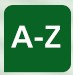
\includegraphics[scale=.6]{glossario}};\end{tikzpicture}}}{\begin{aten}\end{aten}}
    \tcblower
    #1
    \vspace{0.2cm}
\end{mybox}}


% MULTIMIDIA %
\newcommand{\midia}[1]{
\vspace{0.5cm} \begin{mybox}{\makebox[-2.5pt]{\begin{tikzpicture}[overlay]
\node at (0pt,0pt){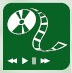
\includegraphics[scale=.6]{midia}};\end{tikzpicture}}}{\begin{aten}\end{aten}}
    \tcblower
    #1
    \vspace{0.2cm}
\end{mybox}}



% ATIVIDADES %
\newcommand{\atividade}[1]{
\vspace{0.5cm} \begin{mybox}{\makebox[-2.5pt]{\begin{tikzpicture}[overlay]
\node at (0pt,0pt){
\includegraphics[scale=.6]{atividade}};\end{tikzpicture}}}{\begin{aten}\end{aten}}
    \tcblower
    #1
    \vspace{0.2cm}
\end{mybox}}


% PAGINA EM BRANCO %
\def\blankpage{%
      \clearpage%
      \thispagestyle{empty}%
      \addtocounter{page}{-1}%
      \null%
      \clearpage}
      
% NOVOS COMANDOS %
\let\parte\part
\let\capitulo\chapter
\let\secao\section
\let\subsecao\subsection
\let\subsubsecao\subsubsection


 % Aqui estão todas as bibliotecas e definições

%---------------------------------------------------------------------
% Início do Documento  
\begin{document}

\renewcommand{\contentsname}{Sumário}
\renewcommand\indexname{Índice}


%-----------------------------------------------------------------------
%	CAPA
%-----------------------------------------------------------------------

% Entrar no arquivo "capa.tex" e modificar "Nome da Disciplina"

\begingroup

\thispagestyle{empty} % Sem Cabeçalho e Rodapé

\begin{tikzpicture}[remember picture,overlay]
\node[inner sep=0pt] (background) at (current page.center) {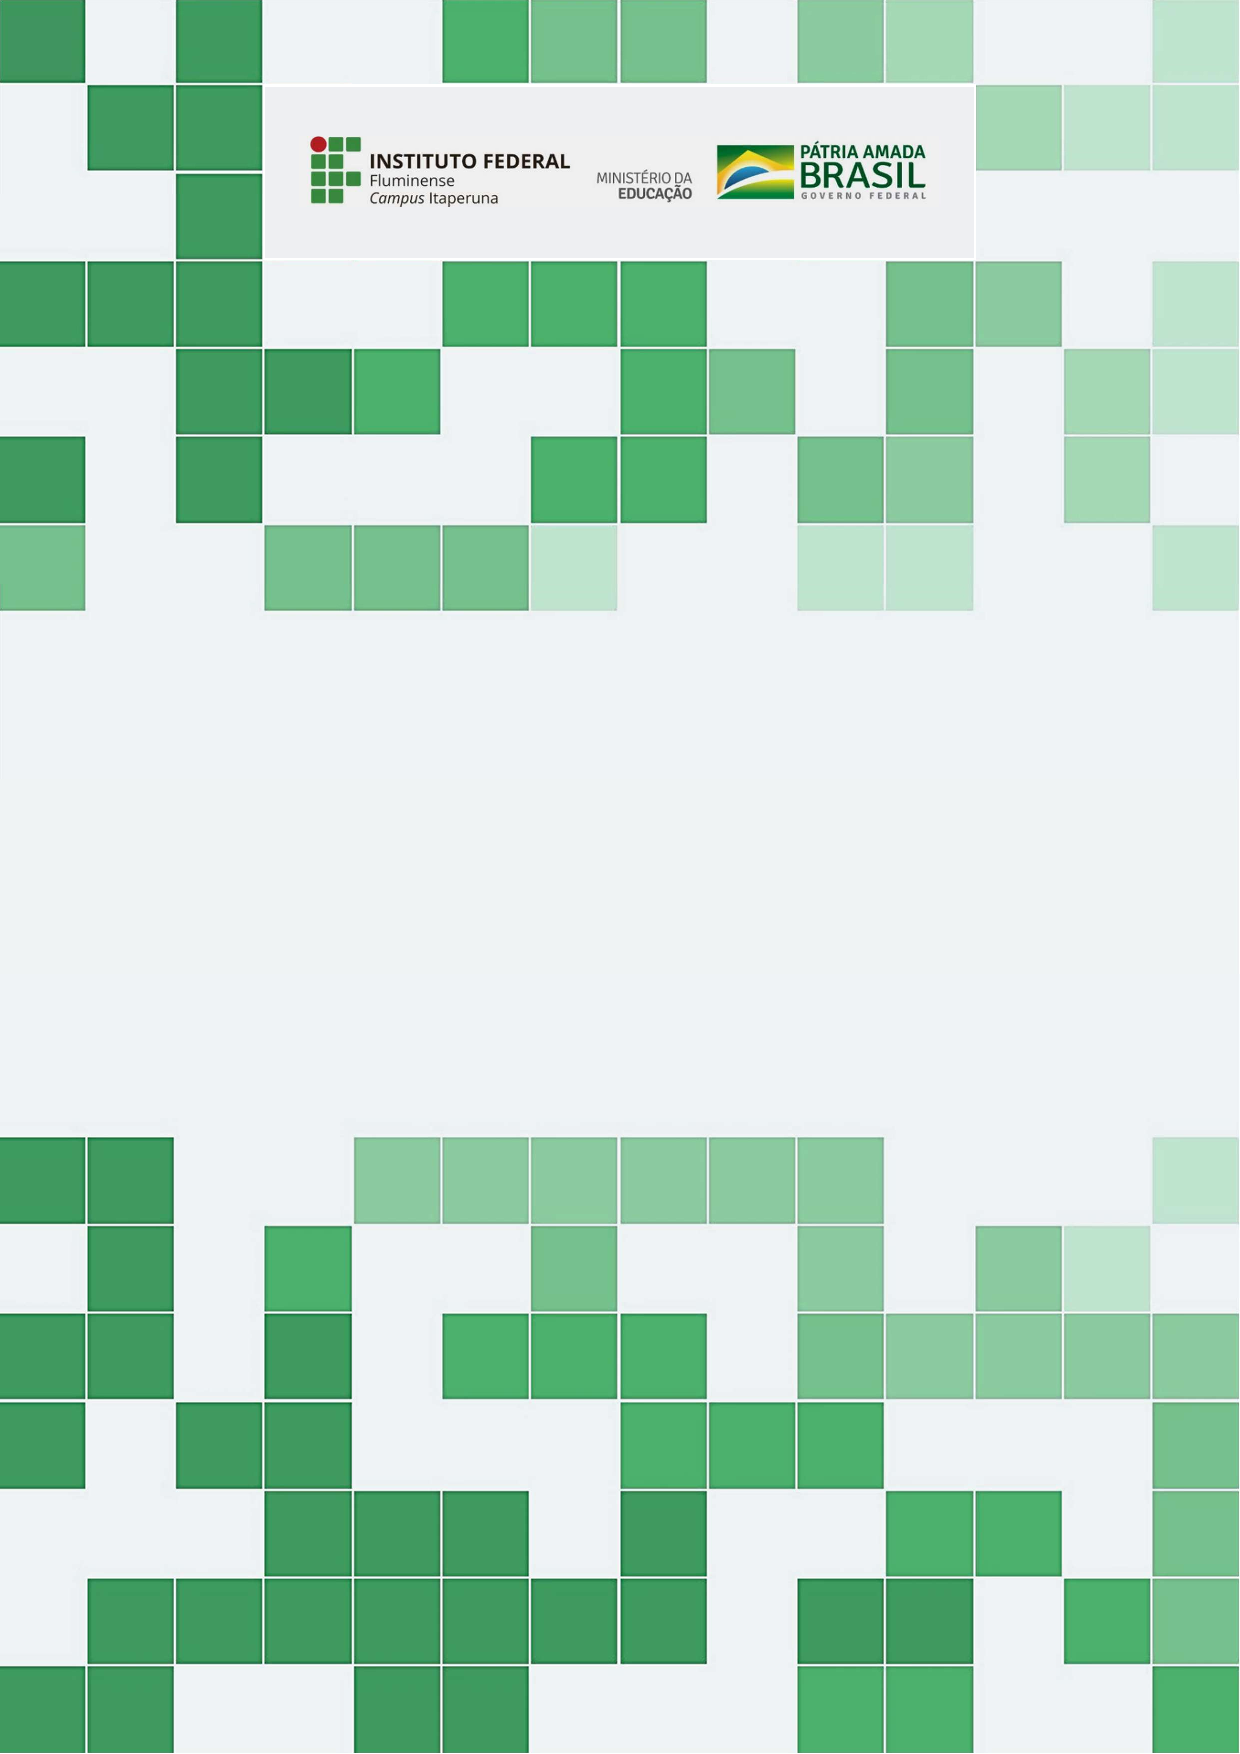
\includegraphics[width=\paperwidth]{Pictures/background.pdf}};
\draw (current page.center) node [fill=ocre!30!white,fill opacity=0.6,text opacity=1,inner sep=1cm]{\color{chapterhead}\Huge\centering\bfseries\sffamily\parbox[c][][t]{\paperwidth}{\centering Nome da Disciplina\\[15pt] % Nome da Matéria
{\Large Apostila Didática}\\[20pt]
% {\huge Prof. Nome do Professor }
}};
\end{tikzpicture}

\vfill

\endgroup




%---------------------------------------------------------------------
%	Página de Apresentação 
%---------------------------------------------------------------------

% Entrar no arquivo "aparesentacao.tex" e redigir o texto de apresentação da disciplina

\cleardoublepage
\newpage
~\vfill
\thispagestyle{empty}
\doublespacing 
\noindent \textsc{Curso Técnico em Eletrotécnica, Instituto Federal Fluminense - Campus Itaperuna}\\

\noindent 
Caro estudante,

Bem-vindos à disciplina de Meio Ambiente e Energias Renováveis que tratará [...] para aprofundar seus conhecimentos sobre [...] no curso Técnico em Eletrotécnica do Instituto Federal Fluminense – Campus Itaperuna.

Para que seu estudo se torne proveitoso e prazeroso, esta disciplina foi organizada em [...] capítulos, com temas e subtemas que, por sua vez, são subdivididos em seções (tópicos), atendendo aos objetivos do processo de ensino-aprendizagem.
O capítulo 1, que trata [...], procuraremos compreender [...].  No capítulo 2, descreveremos
[...]. No capítulo 3, detalharemos [...]. Finalmente, no capítulo 4 refletiremos um pouco sobre [...]. Esperamos que, até o final da disciplina vocês possam:
- Ampliar a compreensão sobre [...];
- Conhecer [...];
- Identificar os aspectos [...];
- Compreender a importância [...];
Para tanto, a metodologia das aulas [...].

Porém, antes de iniciar a leitura, gostaríamos que vocês parassem um instante para refletir sobre algumas questões [...].
Não se preocupe.  Não queremos que vocês respondam de imediato todas essas questões.  Mas esperamos que, até o final, vocês tenham respostas e também formulem outras perguntas.

Vamos, então, iniciar nossas aulas? Bons estudos!


\vspace{3cm}
\DTMlangsetup{showdayofmonth=false}
\noindent \textit{1ª Ed., \today }
\DTMlangsetup{showdayofmonth=true}

%---------------------------------------------------------------------
%	SUMÁRIO
%---------------------------------------------------------------------

% Não é necessário fazer modificação

\chapterimage{capitulo.png}
\pagestyle{empty}
\tableofcontents
\cleardoublepage
\pagestyle{fancy}


%-------------------------------------------------------------
%	INSTRUÇÕES
%-------------------------------------------------------------
%
% A partir deste ponto serão inseridos os capítulos da apostila através dos seguintes passos:
% 
% 1) Incluir um mini resumo de uma parte do documento com o comando "\parte{Nome da Parte}". (Opcional)
% 2) Adicionar uma nova pasta 
% 2) Incluir um capítulo com o comando "\input{"Caminho do Capítulo"}. Ex.: Caso queira incluir o capítulo 1 inserir o comando "\input{Capitulo 1/capitulo}".
% 
%-------------------------------------------------------------
%	DIVISÃO POR PARTES
%-------------------------------------------------------------

\parte{Parte Um}  % Comente essa linha (ctrl+/) se não quiser dividir a apostila em partes
% Título do capítulo
\capitulo{Escreva o título do capítulo aqui} \label{cap1}

  Aqui fica o texto introdutório do capítulo.
  Este é o texto de um capítulo.



\secao{Titulo da seção}\index{seção} % Adiciona  capítulo na parte 1. Para escrever o capítulo 1, abra o arquivo "/Capitulo 1/capitulo1.tex". O mesmo raciocínio vale para os demais.
% Título do capítulo
\capitulo{Escreva o título do capítulo aqui} \label{cap2}

  Aqui fica o texto introdutório do capítulo.
  Este é o texto de um capítulo.



\secao{Titulo da seção}\index{seção}


\parte{Parte Dois}  % Comente essa linha (ctrl+/) se não quiser dividir a apostila em partes
% Título do capítulo
\capitulo{Escreva o título do capítulo aqui}\label{cap3}

  Aqui fica o texto introdutório do capítulo.
  Este é o texto de um capítulo.



\secao{Titulo da seção}\index{seção} % Adicionar  capítulo na parte 2
%% Título do capítulo
\capitulo{Escreva o título do capítulo aqui}\label{cap4}

  Aqui fica o texto introdutório do capítulo.
  Este é o texto de um capítulo.



\secao{Titulo da seção}\index{seção}

% Capítulo com exemplos de comandos, comente quando quiser esconder no seu texto
%--------------------------------------------------------------
%  Capítulos e seções
%--------------------------------------------------------------
%
% Um capítulo se inicia com o seguinte comando "\capitulo{Título}."
%
% Uma seção se inicia com o seguinte comando "\secao{Título da Seção}". Caso queira adicionar a seção ao índice acrescente o comando "\index{Título da Seção}. 
%
% O mesmo princípio é utilizado para os subníveis da seção. São eles: subseção e subsubseção, dados pelos comandos "\subsecao{Título}" e "\subsubsecao{Título}". Estes podem ser seguidos ou não do comando "\index{Título}"
%
%--------------------------------------------------------------



% Título do capítulo
\capitulo{Exemplos}


  Aqui fica o texto introdutório do capítulo.
  Este é o texto de um capítulo.

    % título da seção
    \secao{titulo da seção}\index{Palavra-chave}
 
        Escreva o texto da seção aqui. 
    
    
        % título da subseção
        \subsecao{titulo da subseção}
                
                Texto da seção.
        
                % título da subsubseção
                \subsubsecao{titulo da subseção}\index{palavra-chave(seção)!palavra-chave} 

                    Texto da subsubseção.

%--------------------------------------------------------------
%   Teoremas
%--------------------------------------------------------------


    \secao{Teoremas}\index{Teoremas}

        Esta seção traz exemplos de teoremas.

        \subsecao{Várias Equações}\index{Teoremas!Várias Equações}

            Exemplo de Teorema com várias equações.

            \begin{theorem}[Nome do teorema]
                In $E=\mathbb{R}^n$ all norms are equivalent. It has the properties:
                \begin{align}
                    & \big| ||\mathbf{x}|| - ||\mathbf{y}|| \big|\leq || \mathbf{x}- \mathbf{y}||\\
                    &  ||\sum_{i=1}^n\mathbf{x}_i||\leq \sum_{i=1}^n||\mathbf{x}_i||\quad\text{where $n$ is a finite integer}
                \end{align}
            \end{theorem}

        \subsecao{Linha Única}\index{Teoremas!Linha Única}
            Teorema em Linha Única.
            \begin{theorem}
                A set $\mathcal{D}(G)$ in dense in $L^2(G)$, $|\cdot|_0$. 
            \end{theorem}

%--------------------------------------------------------------


%--------------------------------------------------------------
%   Definições
%--------------------------------------------------------------
\secao{Definições}\index{Definições}

    Exemplo de Definição.
    \begin{definition}[Nova Definição]
        Given a vector space $E$, a norm on $E$ is an application, denoted $||\cdot||$, $E$ in $\mathbb{R}^+=[0,+\infty[$ such that:
        \begin{align}
            & ||\mathbf{x}||=0\ \Rightarrow\ \mathbf{x}=\mathbf{0}\\
            & ||\lambda \mathbf{x}||=|\lambda|\cdot ||\mathbf{x}||\\
            & ||\mathbf{x}+\mathbf{y}||\leq ||\mathbf{x}||+||\mathbf{y}||
        \end{align}
    \end{definition}

%--------------------------------------------------------------

%--------------------------------------------------------------
%   Notações
%--------------------------------------------------------------
\secao{Notações}\index{Notações}

    \begin{notation}
        Given an open subset $G$ of $\mathbb{R}^n$, the set of functions $\varphi$ are:
        \begin{enumerate}
            \item Bounded support $G$;
            \item Infinitely differentiable;
        \end{enumerate}
        a vector space is denoted by $\mathcal{D}(G)$. 
    \end{notation}

%--------------------------------------------------------------



%--------------------------------------------------------------
%  Indicação de ícones
%--------------------------------------------------------------
    \secao{Indicação de Ícones}\index{Indicação de Ícones}

        \mais{ Oferece novas informações que enriquecem o assunto ou “curiosidades” e notícias recentes relacionadas ao tema estudado. Não indicar simplesmente livros, filmes, links, etc. Oriente os estudantes sobre o que vão encontrar no material indicado.
        }

        \midia{ Sempre que se desejar que os estudantes desenvolvam atividades empregando diferentes mídias: vídeos, filmes, jornais, ambiente AVA, sites e outras.
        }

        \glossario{ Indica a definição de um termo, palavra ou expressão utilizada no texto.
        }

        \atividade{ Apresenta atividades em diferentes níveis de aprendizagem para que o estudante possa realizá-las e conferir o seu domínio do tema estudado.
        }

        \atencao{  Indica pontos de maior relevância no texto.
       
        o 
        
        quadro 
       
        aumenta automaticamente
      
        kkk
        }

%--------------------------------------------------------------


%--------------------------------------------------------------
%   Proposições
%--------------------------------------------------------------
    \secao{Proposições}\index{Proposições}

    Estes são exemplos de proposição.
    
        \subsecao{Várias Equações}\index{Proposições!Várias Equações}
            Exemplo com várias equações.
            \begin{proposition}[Nome da Proposição]
                It has the properties:
                \begin{align}
                    & \big| ||\mathbf{x}|| - ||\mathbf{y}|| \big|\leq || \mathbf{x}- \mathbf{y}||\\
                    &  ||\sum_{i=1}^n\mathbf{x}_i||\leq \sum_{i=1}^n||\mathbf{x}_i||\quad\text{where $n$ is a finite integer}
                \end{align}
            \end{proposition}

        \subsecao{Linha Única}\index{Proposições!Linha Única}
            Exemplo em Linha única.
            \begin{proposition} 
                Let $f,g\in L^2(G)$; if $\forall \varphi\in\mathcal{D}(G)$, $(f,\varphi)_0=(g,\varphi)_0$ then $f = g$. 
            \end{proposition}

%--------------------------------------------------------------

%--------------------------------------------------------------
%   Equações 
%--------------------------------------------------------------
    \secao{Equações}\index{Equações}
        Este é um exemplo de uma equação.
        \begin{equation}
            \cos^{2}{x} + \sin^{2}{x} = 1, \quad \forall x \in \mathbb{R}
            \label{equ:1}
        \end{equation}
        
        A equação \ref{equ:1} está referenciada.
        
        Caso não queira uma numeração para a equação:
        \begin{equation*}
            \cos^{2}{x} + \sin^{2}{x} = 1, \quad \forall x \in \mathbb{R}
        \end{equation*}       
        %Note a existência de funções como "\cos{}" e "sin{}" e não, simplismente escrito "cos()" e "sin()".
        
        Um conjunto de equações:
        
        \begin{equation}
            f(x) = 
            \begin{cases}
                2x+1, \quad  x \leq 0 \\
               x^2 +\frac{3}{2}x +\log{x},  \quad  x > 0
            \end{cases}
            \label{equ:2}
        \end{equation}   
        %Note como é criada uma fração com o comando "\frac{}{}"
        
  
       \subsecao{Matrizes}\index{Equações!Matriz}
        
         Exemplo padrão % o símbolo "&" é o separador de colunas e o "\\" indica final de linha
        
        $ %Entrando no Modo matémático entre "$$"
        \begin{bmatrix}
            1 & 2 & 3\\
            a & b & c
        \end{bmatrix}
        $
            Exemplo de equação matricial.
            \begin{equation}
                \begin{bmatrix}
                    Y_{1,1}\\ 
                    \vdots \\   
                    \vdots \\ 
                    Y_{m,1}
                \end{bmatrix}
                =\begin{bmatrix}
                    A_{1,1} & \ldots & \ldots & A_{1,n}\\ 
                    \vdots & \ddots &  & \\   
                    \vdots &  & \ddots  & \\ 
                    A_{m,1}&  &  & A_{m,n}
                \end{bmatrix}
                .\begin{bmatrix}
                    \mathbf{X_{1,1}} \\  %Negrito 
                    \mathbf{\vdots} \\   
                    \mathbf{\vdots} \\ 
                    \mathbf{X_{m,1}}
                \end{bmatrix}
                +\begin{bmatrix}
                    B_{1,1} \\ 
                    \vdots \\   
                    \vdots \\ 
                    B_{m,1}
                \end{bmatrix}
            \end{equation}


        Exemplos de outros modelos de matrizes 
        \url{https://pt.overleaf.com/learn/latex/Matrices}
      

      

%--------------------------------------------------------------
%   Exemplos 
%--------------------------------------------------------------
    \secao{Exemplos}\index{Exemplos}

        Este é um exemplo de exemplos.
        
        \subsecao{Equações e Texto}\index{Exemplos!Equações e Texto}
            \begin{example}
                Let $G=\{x\in\mathbb{R}^2:|x|<3\}$ and denoted by: $x^0=(1,1)$; consider the function:
                \begin{equation}
                    f(x)=\left\{\begin{aligned} & \mathrm{e}^{|x|} & & \text{si $|x-x^0|\leq 1/2$}\\
                    & 0 & & \text{si $|x-x^0|> 1/2$}\end{aligned}\right.
                \end{equation}
                The function $f$ has bounded support, we can take $A=\{x\in\mathbb{R}^2:|x-x^0|\leq 1/2+\epsilon\}$ for all $\epsilon\in\intoo{0}{5/2-\sqrt{2}}$.
            \end{example}
        \subsecao{Parágrafo de Texto}\index{Exemplos!Parágrafo de Texto}
            \begin{example}[Nome do Exemplo]
                \lipsum[2]
            \end{example}

%--------------------------------------------------------------

%--------------------------------------------------------------
%   Exercícios
%--------------------------------------------------------------
    \secao{Exercícios}\index{Exercícios}

        Exemplo de exercício.
        \begin{exercise}
            This is a good place to ask a question to test learning progress or further cement ideas into students' minds.
        \end{exercise}

%--------------------------------------------------------------


%--------------------------------------------------------------
%   Problemas
%--------------------------------------------------------------
    \secao{Problemas}\index{Problemas}
        \begin{problem}
            Qual é o sentido do mundo?
        \end{problem}

%--------------------------------------------------------------



%--------------------------------------------------------------
%--------------------------------------------------------------
%  Nota de rodapé
%--------------------------------------------------------------
 \secao{Nota de rodapé}\index{Rodapé}

        Notas de rodapé são legais para informações extras\footnote{Exemplo de nota de rodapé}.


%--------------------------------------------------------------
%   Listas 
%--------------------------------------------------------------
    \secao{Listas}\index{Listas}

        Listas são úteis para apresentar informção de maneira concisa e ordenada.

        \subsecao{Lista Numerada}\index{Listas!Lista Numerada}

            \begin{enumerate}
                \item The first item
                \item The second item
                \item The third item
            \end{enumerate}

        \subsecao{Bolinhas}\index{Listas!Bullet Points}

            \begin{itemize}
                \item The first item
                \item The second item
                \item The third item
            \end{itemize}

Observação: tem como mudar de bolinha para outros símbolos, pergunte ao Rodolfo.

\secao{Listas aninhadas1}\index{Listas!Lista Aninhada}

\begin{enumerate}
   \item topico 1
     \begin{itemize}
         \item subitem 1
         \item subitem 2
      \end{itemize}
   \item topico 2
       \begin{itemize}
         \item subitem 1
         \item subitem 2
       \end{itemize}
\end{enumerate}


Outros exemplos de listas aqui \url{https://pt.overleaf.com/learn/latex/Lists}

%--------------------------------------------------------------


%--------------------------------------------------------------
%   Tabelas
%--------------------------------------------------------------
    \secao{Tabelas}\index{Tabelas}

        Para criar tabelas facilmente \href{https://www.tablesgenerator.com/}{\textbf{Clique Aqui}}

        %% INÍCIO DA TABELA %%
        \begin{table}[h]  %-- Início da Tabela
            %-- Legenda e Referências --%%
            \caption{Legenda Tabela}
            \label{tab:exemplo}             % comando para permitir citar a tabela
            \addcontentsline{toc}{table}{Tabela \ref{tab:exemplo}}

            %-- Corpo da Tabela --%
            \centering
            \begin{tabular}{l l l}
                \toprule
                \textbf{tópico 1} & \textbf{Valor 2} & \textbf{Valor 3}\\
                \midrule
                A 1 & 0.0003262 & 0.562 \\
                B 2 & 0.0015681 & 0.910 \\
                C 3 & 0.0009271 & 0.296 \\
                \bottomrule
            \end{tabular}
        \end{table}  %-- Fim da Tabela
        %% FIM TABELA %%


%---------------------------------------------------------------
%   Citação de tabela 
%---------------------------------------------------------------

    Como referenciar à Tabela  \ref{tab:exemplo} no texto automaticamente.

%--------------------------------------------------------------


%--------------------------------------------------------------
%  Figuras
%--------------------------------------------------------------
    \secao{Figuras}\index{Figuras}

        Aqui será acrescentada uma figura.
        % Para adicionar uma figura, copie o código abaixo e substitua o caminho "capitulo exemplos/Imagens/exemplo_figura.jpg" pelo nome da figura desejada, escolhendo-a nas opções que aparecerão. Outros formatos além do .jpg são suportados, na dúvida só testar.
        %
        % Caso queira modificar o tamanho da imagem, altere o valor "0.3" para o desejado. Este valor representa a porcentagem do espaço de uma linha.
        %
        % Para referenciá-la no texto, dê um nome único para o argumento "fig:ref" do comando \label{}, por ex.: \label{fig:motor1.jpg}

        \begin{figure}[htbp!]
            \centering
            
\includegraphics[width=0.3\textwidth]{capitulo exemplos/Imagens/exemplo_figura.jpg}
            \caption{Legenda da Figura}
            \label{fig:ref}
        \end{figure}

%--------------------------------------------------------------
%   Citação de Figuras
%--------------------------------------------------------------
% O comando \ref{nome que esta no label} irá gerar o numero da figura automaticamente

Como mostrado na Figura \ref{fig:ref}, ....


%--------------------------------------------------------------



%--------------------------------------------------------------
% Figuras lado a lado
%--------------------------------------------------------------
        \subsecao{Figuras}\index{Figuras!Figuras lado a lado}
            
            Segue um exemplo de imagens lado a lado

            %Caso deseje adicionar uma figura embaixo de outra, modifique o valor "0.4" na propriedade "width" do comando "\includegraphics", em ambas as figuras, para um valor maior.

            \begin{figure}[H]
                \centering
                \subfigure[Legenda A]{
                    
\includegraphics[width=0.4\textwidth]{capitulo exemplos/Imagens/exemplo_figura.jpg}
                    \label{fig:ref1}
                }
                \hfill
                \subfigure[Legenda B]{
                    
\includegraphics[width=0.4\textwidth]{capitulo exemplos/Imagens/exemplo_figura.jpg}
                    \label{fig:ref2}
                }
                \caption{Legenda das duas Figuras}
                \label{fig:ref3}
            \end{figure}
            
            Apontando para as subfiguras \ref{fig:ref1} e \ref{fig:ref2} da imagem \ref{fig:ref3}.


            Alterando o valor da propriedade "width" para "0.5", teremos o seguinte efeito:
            \begin{figure}[H]
                \centering
                \subfigure[Legenda A]{
                    
\includegraphics[width=0.5\textwidth]{capitulo exemplos/Imagens/exemplo_figura.jpg}
                    \label{fig:ref4}
                }
                \hfill
                \subfigure[Legenda B]{
                    
\includegraphics[width=0.5\textwidth]{capitulo exemplos/Imagens/exemplo_figura.jpg}
                    \label{fig:ref5}
                }
                \caption{Legenda das duas Figuras}
                \label{fig:ref6}
            \end{figure}      

            Para 3 figuras:
        
            \begin{figure}[H]
                \centering
                \subfigure[Legenda A]{
                    
\includegraphics[width=0.3\textwidth]{capitulo exemplos/Imagens/exemplo_figura.jpg}
                    \label{fig:ref7}
                }
                \hfill
                \subfigure[Legenda B]{
                    
\includegraphics[width=0.3\textwidth]{capitulo exemplos/Imagens/exemplo_figura.jpg}
                    \label{fig:ref8}
                }
                \hfill
                \subfigure[Legenda C]{
                    
\includegraphics[width=0.3\textwidth]{capitulo exemplos/Imagens/exemplo_figura.jpg}
                    \label{fig:ref9}
                }
                \caption{Legenda das duas Figuras}
                \label{fig:ref10}
            \end{figure}
            
            %   Lembre-se que o conteúdo nos comandos "\label{}" devem ser únicos para o referenciamento correto de cada imagem/subimagem.
        
%--------------------------------------------------------------
% Citação de referência bibliográfica
%--------------------------------------------------------------
\secao{Citação de referência bibliográfica}\index{Referência}

Segundo \cite{sobrenome_id}, é assim que cita uma referência no \LaTeX.


%--------------------------------------------------------------
% Citação de capítulo
%--------------------------------------------------------------
\secao{Citação de capítulo}\index{Citação de Capítulo}


Citação do capítulo \ref{cap1} , capítulo \ref{cap3}, ...., é o mesmo esquema para imagens e tabelas.


%--------------------------------------------------------------
%   Corolários
%--------------------------------------------------------------
    \secao{Corolários}\index{Corolários}

        Exemplo de Corolário
        \begin{corollary}[Corollary name]
            The concepts presented here are now in conventional employment in mathematics. Vector spaces are taken over the field $\mathbb{K}=\mathbb{R}$, however, established properties are easily extended to $\mathbb{K}=\mathbb{C}$.
        \end{corollary}

%--------------------------------------------------------------



%--------------------------------------------------------------
%   Descrição
%--------------------------------------------------------------

        \subsecao{Descrição e Definições}\index{Listas!Descrição e Definições}

            \begin{description}
                \item[Name] Description
                \item[Word] Definition
                \item[Comment] Elaboration
            \end{description}
%--------------------------------------------------------------

%--------------------------------------------------------------
%   Vocabulário
%--------------------------------------------------------------
    \secao{Vocabulário}\index{Vocabulário}

        Define a word to improve a students' vocabulary.

        \begin{vocabulary}[Palavra]
            Definição da palavra.
        \end{vocabulary} 

%-----------------------------------------------------------------
%	BIBLIOGRAFIA
%-----------------------------------------------------------------

\capitulo*{Bibliografia}
\addcontentsline{toc}{chapter}{\textcolor{ocre}{Bibliografia}} \nocite{*}
% Adiciona a Bibliografia para o Sumário

%------------------------------------------------
%   Artigos
%------------------------------------------------

\secao*{Artigos}
\addcontentsline{toc}{section}{Artigos}
\printbibliography[heading=bibempty,type=article]

%------------------------------------------------
%   Livros
%------------------------------------------------

\secao*{Livros}
\addcontentsline{toc}{section}{Livros}
\printbibliography[heading=bibempty,type=book]

%------------------------------------------------
%   Manuais
%------------------------------------------------

\secao*{Manuais}
\addcontentsline{toc}{section}{Manuais}
\printbibliography[heading=bibempty,type=manual]

%------------------------------------------------
%   Sites
%------------------------------------------------

\secao*{Sites}
\addcontentsline{toc}{section}{Sites}
\printbibliography[heading=bibempty,type=misc]


%---------------------------------------------------------------
%	ÍNDICE
%---------------------------------------------------------------

\cleardoublepage 
\phantomsection
\setlength{\columnsep}{0.75cm} 
\addcontentsline{toc}{chapter}{\textcolor{ocre}{Índice}} 
\printindex 
%---------------------------------------------------------------

\end{document}

%Fim do Documento 